%Edit 9991 ZZZ to report number nnnn 
%Edit 9.9.1 YYMILE to milestone number m.m.m
%Edit Finite elements for finite difference modellers YYTITLE to report title - Words Start with Caps
\documentclass[11pt,twoside,a4paper]{article}
%%======================================================================
%% PACKAGES:
%%
%\usepackage{times}               % Times+Helvetica+Courier fonts
\usepackage{helvet}              % helvetica + cmr
\usepackage{fancyhdr}       % package for headers/footers
\usepackage{amsmath}
\usepackage{amssymb}
\usepackage{graphicx}            % Graphics.
%\usepackage{a4}                  % page layout to fit A4
%\usepackage{lastpage}            % get page no of last page
%\usepackage{ifthen}              % logical branching
%\usepackage{showkeys}              % show labels
\usepackage{hyperref}            %insert hyper-links
\usepackage{latexsym}
% uncomment the following to override auto page total
%\pptotal{20}
%%======================================================================

% ensure sans-serif font used throughout
\renewcommand{\familydefault}{\sfdefault}

\newcommand{\culhamissueno}{1.00}%<==edit
\newcommand{\culhamshorttitle}{CD/EXCALIBUR-FMS/9991}%<==edit
\newcommand{\Sec}[1]{Section~\ref{sec:#1}}
\newcommand{\Fig}[1]{Figure~\ref{fig:#1}}
\newcommand{\Eq}[1]{Equation~(\ref{eq:#1})}
\newcommand{\Eqs}[2]{Equations(\ref{eq:#1}) and~(\ref{eq:#2})}
\newcommand{\Figs}[2]{Figures~\ref{fig:#1}--~\ref{fig:#2}}
%Bold lc for script names, tt for computer code and file-names
%\F{NEPTUNE} always in caps
\newcommand{\F}[1]{\textsc{#1}}
\newcommand{\B}[1]{\textbf{#1}}
\newcommand{\T}[1]{{\tt #1}}
\newcommand{\V}[1]{\mathbf{#1}}
\newcommand{\I}[1]{\textit{#1}}
\newcommand{\nep}{\textsc{NEPTUNE}}
\newcommand{\exc}{\textsc{E}x\textsc{CALIBUR}}


%%======================================================================

%% REPORT COVER PAGE Information


%%QA BOX information -- change following as needed
\newcommand{\culhamboardname}{Martin O'Brien}%<==edit
\newcommand{\culhamcontactname}{Rob Akers}%<==edit
\newcommand{\culhamauthor}{Wayne Arter}%<==edit
\newcommand{\culhamauthora}{Lucian Anton}%<==edit
\newcommand{\culhamauthorb}{Debasmita Samaddar}%<==edit
%\newcommand{\culhamcontacttel}{Telephone: 01235 466498}
%\newcommand{\culhamcontactemail}{Email: rob.akers@ukaea.uk}

\newcommand{\culhamdate}{\today}%<=edit
\newcommand{\culhamdatea}{\today}%<=edit
\newcommand{\culhamdateb}{\today}%<=edit

% reproduce Rob's page size

\setlength{\textheight}{220.0mm}
\setlength{\textwidth}{165.0mm}
\setlength{\topmargin}{0.0mm}
\setlength{\oddsidemargin}{0.0mm}
\setlength{\evensidemargin}{\oddsidemargin}
\setlength{\parindent}{0mm}
\addtolength{\parskip}{0.5\baselineskip}
\setlength{\topsep}{0pt}
\setlength{\itemsep}{0pt}

%%======================================================================
\begin{document}

%Titlepage comes out wrong size, but should look right apart from
% picture which cannot be wider than c.150mm.
% To produce conforming report rp1pub.pdf
% remove title page by commenting out lines ending in %<==omit, then
% sed -e '/<==omit$/s/^/%/' < rp1.tex > rp1omit.tex
% pdflatex rp1omit;bibtex rp1omit; pdflatex rp1omit
% pdfunite cover.pdf rp1omit.pdf rp1pub.pdf 
%\begin{titlepage}%<==omit
%\vspace*{-30mm}%<==omit
%
\includegraphics[width=2.5cm]{../corpics/cofaplus} \\[2.0\baselineskip]%<==omit
%{\LARGE {\textbf{\textsf{ExCALIBUR}}}}\\[2.0\baselineskip]%<==omit
%{\LARGE \culhamtitle } \\[2.0\baselineskip]%<==omit
%{\textbf{\textsf{Abstract}}}\\%<==omit
\centerline{\Huge Finite elements for finite difference modellers}

The report describes how complex geometry leads naturally to the adoption
of finite element schemes, and explains features of the finite element
approach.

~

\centerline{\Large Wayne Arter \today}
%%The report describes equations for \exc \ project \nep \ \Papp s.  
The numbering of the systems follows that of the \nep\ Science Plan, so 
that those listed under FM-WP2 are denoted 2-1, 2-2, etc., and 
under FM-WP3 as 3-1, 3-2, etc. It is a living document to which further equation 
systems will be added throughout the course of the project.
%<==omit
%%<==omit
%\vfill%<==omit
%\centerline{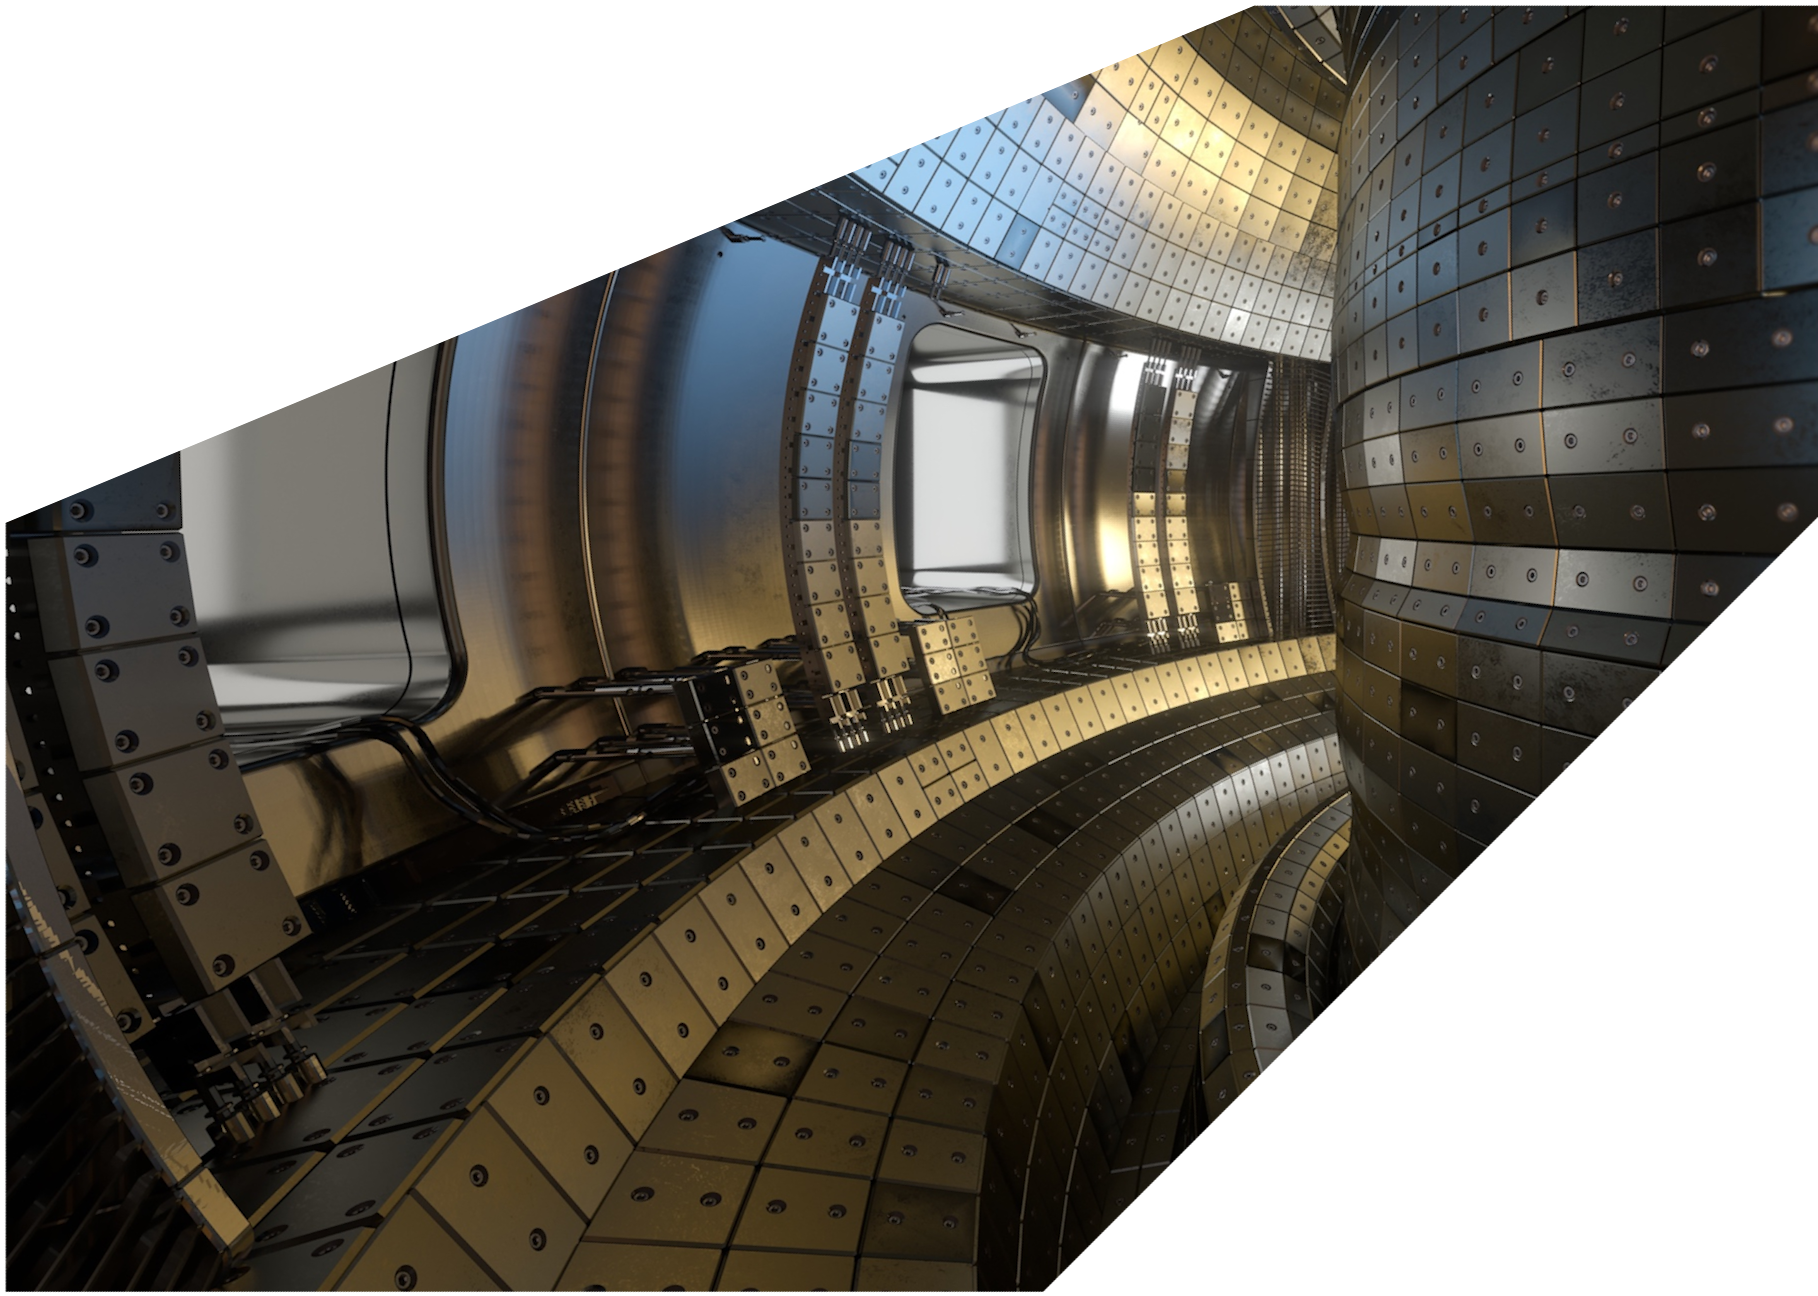
\includegraphics[width=0.9\textwidth]{../corpics/tokintcrop}}%<==omit
%\end{titlepage}%<==omit

%\hspace{-30mm}\begin{table}[h]
\sffamily
\begin{center}
\textbf{\textsf{UKAEA REFERENCE AND APPROVAL SHEET}}
\begin{tabular}{||p{5.7cm}|p{4.7cm}|p{5.0cm}||}
\hline
\hline
& Client Reference: &  \\
\hline
& UKAEA Reference: & \culhamshorttitle \\
& & \\
\hline
& Issue: & \culhamissueno \\
\hline
& Date: & \culhamdateb \\
\hline
\multicolumn{3}{||l||}{} \\
\multicolumn{3}{||l||}{Project Name: ExCALIBUR Fusion Modelling System} \\
\multicolumn{3}{||l||}{} \\
\hline
\end{tabular}
\begin{tabular}{||p{3.3cm}|p{4.6cm}|p{3.5cm}|p{3.6cm}||}
\hline
& Name and Department & Signature & Date \\
\hline
Prepared By: & \culhamauthora & N/A & \culhamdate \\
& \culhamauthor & N/A & \culhamdate \\
%& \culhamauthorb  & N/A & \culhamdate \\
%& \culhamauthorc  & N/A & \culhamdate \\
& & & \\
& BD & & \\
\hline
Reviewed By: & \culhamcontactname & 
\includegraphics[width=3.0cm]{../corpics/blanksign}& \culhamdatea \\
& & & \\
& Advanced Computing Dept. Manager & & \\
\hline
%Approved By: & \culhamboardname  & \includegraphics[width=3.0cm]{../corpics/mobsign} & \culhamdateb \\
%& & & \\
%& MSSC & &\\
%\hline
\hline
\end{tabular}
\end{center}
\end{table}


\clearpage
\section{Introduction}\label{sec:intro}
The edge region is in parts a very good vacuum, so 
that the plasma ion species typically do not thermalise fully.
Nonetheless it may be adequate for many purposes to treat the majority ionised species as fluids,
although this is harder to argue for impurity species that may be present only in relatively
small numbers.
In fact, collision timescales typically vary $\tau\propto T^{3/2}/N$ where $T$ is the temperature of the species
and~$N$ is its number density, so that a species may be treatable as a fluid over say microsecond
timescales in cooler, denser regions, but not on shorter timescales or in parts closer to the core.
There is the additional complication of sheath formation at the edge, where the preferential
loss of electrons leads to strong electric fields and consequently flows close to sonic,
so that most workers model the sheath plasma using particles, typically with the Particle-in-Cell~(PIC)
approach, although for the Vlasov equation a wide range of numerical techniques has been examined,
see eg.\ Palmroth~et~al~\cite[\S\,4]{Pa18Vlas}.
\emph{N.B. Discussion in this note implies usage of particles to model kinetic effects,
not schemes such as SPH designed to model advection of classical fluids.}

The cooler parts of the tokamak edge plasma may contain large numbers of
neutral atoms.
Neutrals are generically less likely than charged species to thermalise.
They circulate into hotter and denser regions and collide with charged species.
Classical transport coefficients~$\kappa$, in
addition to a~$1/\tau$ dependence, are anisotropic because of the strong magnetic field,
to the extent that collisions with neutrals may become an important limiting mechanism
for transport along the field. Operationally the most important aspect of the
neutral species is however that because of the collisions, they
represent a source of plasma.

The non-Maxwellian or kinetic aspects of the edge may lead to a need to solve the
Boltzmann equation, in fact not only with quadratic source terms representing interaction
between two species colliding, but with cubic terms representing chemical reactions.
Classical fluid dynamics of course assumes Maxwellian dependence on phase velocity and
concentrates on the first few moments  density, mean flow and sometimes temperature
as well as pressure. It can be helpful to introduce
the concept of phase-fluid, where extra dimensions represent the velocity-space
dependence at a position in full detail.
In the phase-fluid approach, the concept of multiplicatively perturbing
a Maxwellian has been explored. The main and important advantage of this approach
is that it often facilitates massive simplification of the collision integrals
in Boltzmann, to a single point term in significant cases, eg.\ ref~\cite{zhdanov}.

Kormann, with Yurova and others (private communication, 2019) have recently reviewed the use of 
the Hermite basis (ie.\ a Gaussian multiplied by a Hermite polynomial). Two
significant works are Vencels et al.~\cite{Ve16Spec} describing Spectralplasmasolver
and J.T.Parker's thesis~\cite{jtparker} which describes software focused on
gyroaveraged kinetics, namely SPECTROGK. Note that all these works use a Fourier
representation for real space, the so-called Fourier-Hermite method.
%, so that additional development would be needed for \nep

Even with the simplification of a multiply-periodic domain,
there are nonetheless issues particularly at high velocity values
and of course a Maxwellian may not be a particularly good approximation. 
Hence, borrowing from classical CFD practice on a infinite domain, it might be
interesting to look at mappings which expand a set of compact spectral elements to cover
the whole of velocity space.

\begin{figure}
\centerline{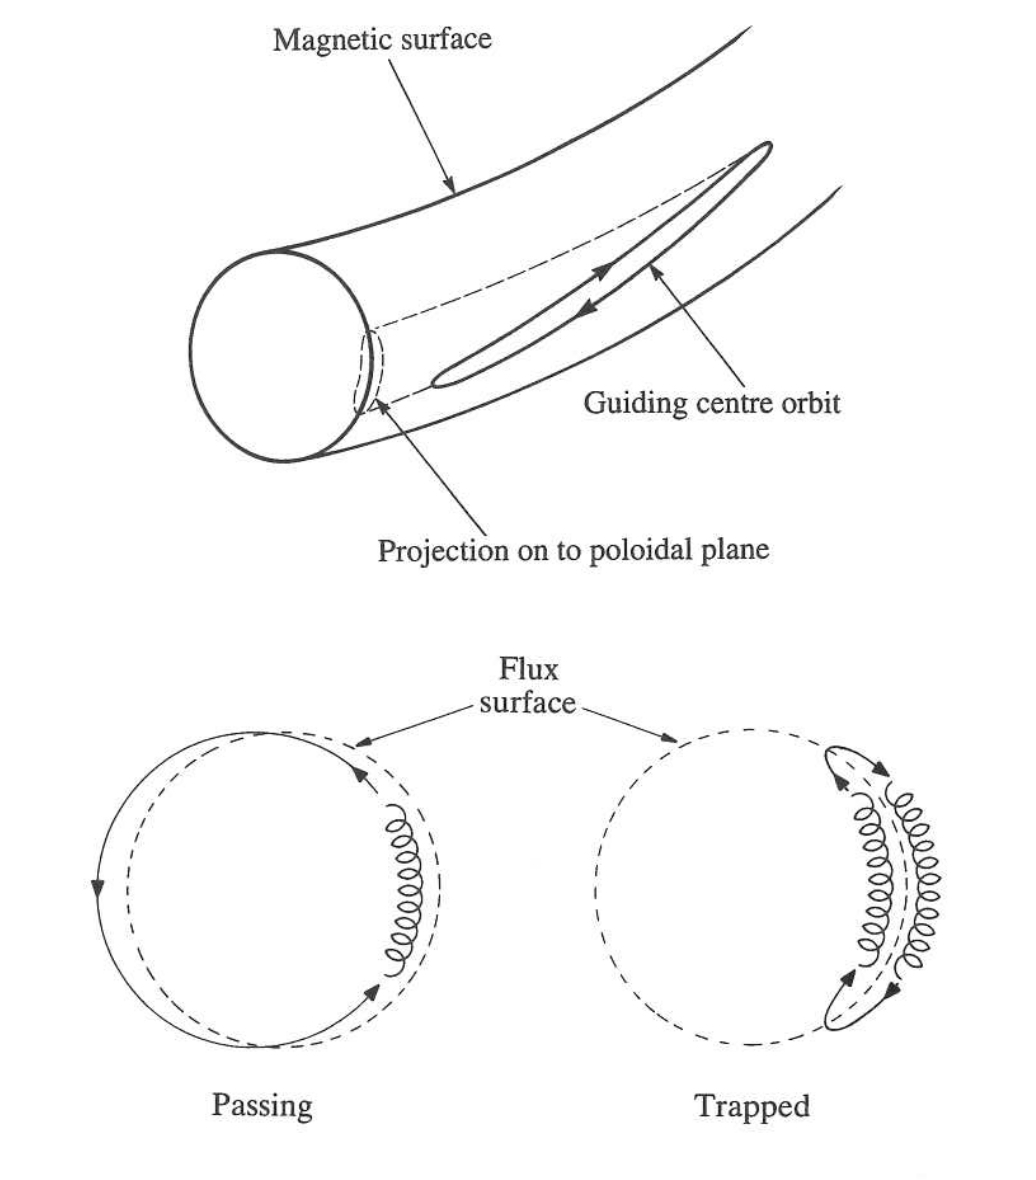
\includegraphics[width=8cm]{../png/pcle_orbits}}
\caption{Important classes of particle trajectories from Wesson~\cite[\S\,3.10]{wesson}.\label{fig:orbits}}
\end{figure}

Alternatively it may be easier to return to basics and look at a particle representation
for the ionised species as well as for the neutrals. This
may be as efficient as using higher order elements since the distribution function in velocity may not be
very smooth. As the sketch in \Fig{orbits} indicates, there are two important classes of particle
trajectories, depending on the particle energy and where in the magnetic field they begin.
The first set approximately follow the fieldlines, gyrating as they go, whereas the second set
may have trajectories that bounce. There is lack of smoothness at the trapped-passing
boundary in velocity space.


%The need to use particle as well as fluid models, puts a significant burden on the software,
%because it gives rise to a general need to be able to move between representations without
%introducing excessive error.

\clearpage
\section{Meshing Issues}\label{sec:meshing}
\subsection{Geometrical Problems}\label{sec:geomprob}
\begin{figure}[h]
\centerline{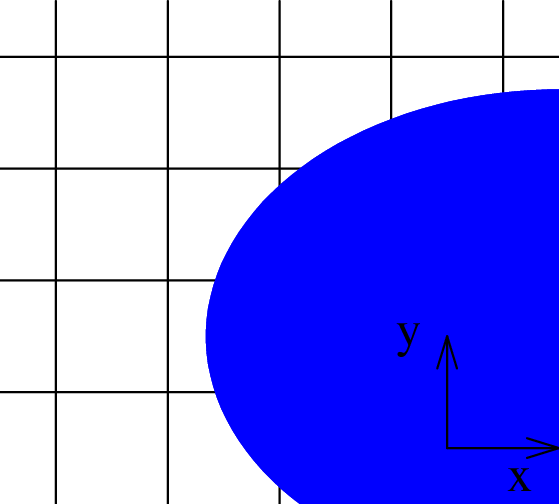
\includegraphics[width=6cm]{../pics/mesh}
\hspace{1cm}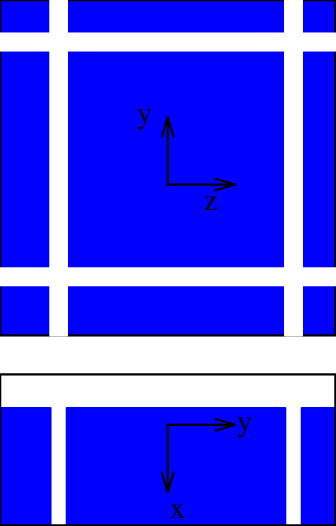
\includegraphics[width=6cm]{../pics/g12}
}
\centerline{(a) \hspace{7cm}(b)}
\caption{Geometries, bodies shown in blue. (a) left, G1~problem of meshing round a simple 2-D geometry, an ellipse
with axes parallel to the coordinate axes $x$~and~$y$ indicated.
%The plot below shows the
%pixellated mesh geometry where the dashed line represents the original ellipse boundary.
(b) right, the G2~problem of meshing in the gaps between solid bodies.
The sketch below
shows a typical slice in a vertical plane aligned with either the $y$ or $z$~axis,
showing a shallow connecting volume above the bodies.
\label{fig:mesh}}
\end{figure}
\Fig{mesh}(a) illustrates the first problem~G1, to mesh around a simple 2-D geometry, an ellipse
with axes parallel to the coordinate axes $x$~and~$y$ indicated.
The mesh sketched in \Fig{mesh} has cells which are exaggeratedly large
but it nonetheless illustrates issues which still arise even for meshes which are much
smaller relative to the geometry.

\paragraph{Physical Issue}
For example, the ellipse
could represent a specially shaped PFC body, so that numerical solution of a heat
transfer problem is required in the exterior region to determine the temperature
distribution on the elliptical surface. Since it involves edge plasma, a numerical 
discretisation is required which may be either explicit or implicit. In the case
of an explicit scheme, the maximum allowed timestep is given by the time taken for
fluid/plasma to flow across the smallest cell. Implicit schemes are less constrained, but
generally have better convergence properties if cell sizes vary smoothly across
the domain of interest.

A second geometry~G2 is illustrated in \Fig{mesh}. This could be a significant extension of 
a larger volume extruded to model heat transfer by plasma in the gaps between the first wall
tiles. Thus numerical calculation is needed only in the area which is shown white in the figure,
which is shown exaggeratedly large compared to the relative inter-tile spacing in most devices.

%\clearpage
\subsection{Cell masking}\label{sec:mask}
\begin{figure}[h]
\centerline{\includegraphics[width=6cm]{../pics/mellpix}
\hspace{1cm}\includegraphics[width=6cm]{../pics/vgapp}
}
\centerline{(a) \hspace{7cm}(b)}
\caption{First meshing considerations.
(a) left, pixellated mesh for the G1~geometry where the dashed line represents the original ellipse boundary.
(b) right, heavy lines indicate possible multiblock boundaries in a vertical plane
for the G2~geometry.
\label{fig:mellpix}}
\end{figure}
For G1, the first approach that might be considered is to identify cells within the surface
geometry and exclude them from the modelling. The natural metric for deciding where
a cell lies is the fraction of body it contains. Taking $0.5$ as the cut-off
gives rise to the pixellated G1~geometry of \Fig{mesh}(a) which will be seen
has one obvious difficulty, namely
how to compute an accurate approximation to the surface normal.

Note that masking already gives rise to a need to consider meshing as a separate issue,
in that finite-difference cells have to be divided into three separate categories depending on whether
they lie entirely inside, outside or intersect the edges of the bodies.  Moreover for the
last category, the area of cell inside the body has somehow to be computed accurately.

%\clearpage
\subsection{Multiblock}\label{sec:multiblock}
Problem~G2 illustrates the fact that there is problem with finite difference
meshes even when the geometry has a simple rectilinear form, in that \Fig{mesh}(b)
indicates that, assuming a uniform grid spacing, most of the cells will be inactive.
This leads to the multiblock approach illustrated in \Fig{mellpix}(b), where the mesh is
confined to the white areas surrounded by thick black lines. The problem is that
although each block is cuboidal and might be treated using finite differences in its
interior, there are potential issues at the joins, and the need for a complex data
structure to describe how they interconnect.
%\begin{figure}
%\centerline{\includegraphics[width=6cm]{../pics/vgapp}}
%\caption{The heavy lines indicate possible multiblock boundaries in a vertical plane
%for the G2~geometry.
%\label{fig:vgapp}}
%\end{figure}

\begin{figure}
\centerline{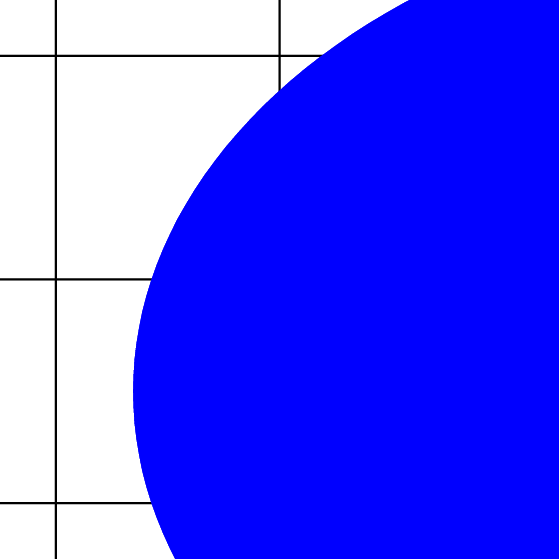
\includegraphics[width=6cm]{../pics/dmesh}
\hspace{1cm}\includegraphics[width=6cm]{../pics/meshabc}
}
\centerline{(a) \hspace{7cm}(b)}
\centerline{\includegraphics[width=6cm]{../pics/fd}
\hspace{1cm}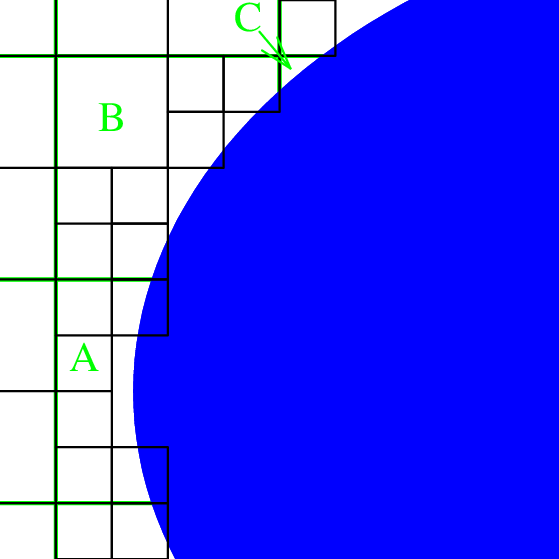
\includegraphics[width=6cm]{../pics/mfenabc}
}
\centerline{(c) \hspace{7cm}(d)}
\caption{(a) and (c) left
At top (a) close-up of the G1~problem of meshing round a simple 2-D geometry, (c)
shows attempted refinement of finite difference mesh.
(b) and (d) right. Close up at bottom (d) of the cells labelled $A$, $B$ and~$C$ at top, showing
a hierarchy of local refinements by a factor~half. Note that refinements by a factor one~quarter
may be excluded by bisecting the larger cell which shares the edge.
\label{fig:mfenabc}}
\end{figure}

\clearpage
\subsection{Mesh refinement}\label{sec:meshref}

\subsubsection{Finite difference mesh refinement}\label{sec:fdmeshref}
In problem~G1, clearly some form of mesh refinement near the boundary is required. \Fig{mfenabc}(a) shows
a close-up of the region near the `nose' of the ellipse, and \Fig{mfenabc}(c) indicates what happens
if the mesh is refined by insertion of extra cells. To preserve the simple $(x,y)$ addressing
structure, it is necessary to insert entire row or columns, even though only a few cells
in a particular column may need refinement. If the scheme is explicit however, this extra
cost is dominated by the fact that since there are cell edges that are one-eighth the
original length, $8$~times as many timesteps are needed to model the same elapsed physical time.
%\begin{figure}
%\centerline{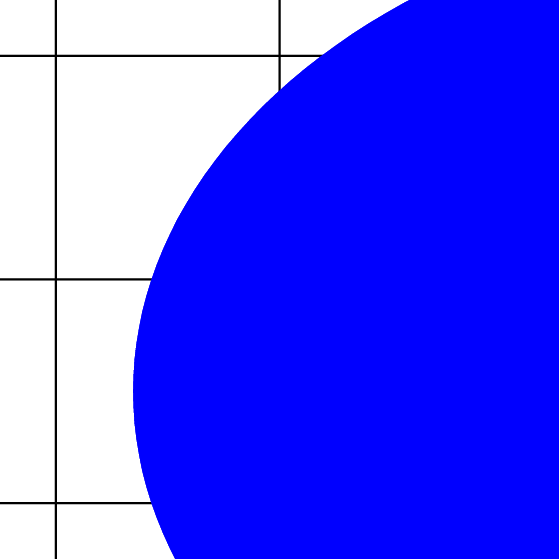
\includegraphics[width=6cm]{../pics/dmesh}}
%\caption{Close-up of the G1~problem of meshing round a simple 2-D geometry, an ellipse
%with axes parallel to the coordinate axes.
%\label{fig:dmesh}}
%\end{figure}
%\begin{figure}
%\centerline{\includegraphics[width=6cm]{../pics/fd}}
%\caption{Refinement of finite difference mesh in the G1~problem.
%\label{fig:fd}}
%\end{figure}

\subsubsection{Hierarchical refinement}\label{sec:hieref}
Another idea is make the cell subdivisions suggested by \Fig{mfenabc}(c) locally. This is illustrated 
in \Fig{mfenabc}(b) and \Fig{mfenabc}(d).
The immediate point to make is that this is \emph{not} a finite-difference mesh, and
addressing the cells shown at right, even though they are each square, will require a
matching hierarchical structure. The problem is worse however because of the so-called
hanging nodes, which occur where larger cells are adjacent to smaller ones, that
require special replacement of the simple finite-difference formulae.

%\clearpage
\subsection{Mapped meshing}\label{sec:mapped}
\begin{figure}[h]
\centerline{\includegraphics[width=6cm]{../pics/basic}
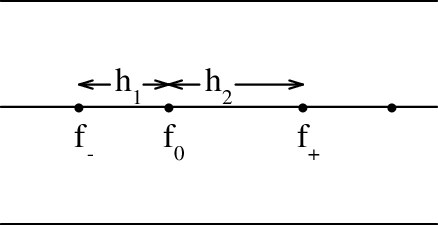
\includegraphics[width=6cm]{../pics/basic2}
}
\caption{A 1-D mapping takes points separated by~$h$ to non-equispaced separation.
\label{fig:basic}}
\end{figure}
With reference to \Fig{basic}(right),
recall the usual approach to deriving finite difference approximation by
means of Taylor series
\begin{eqnarray} \label{eq:taylor}
f_+&=&f_0 + h_2 f'_0 + \frac{1}{2} h_2^2 f^{''}_0 + \frac{1}{6} h_2^3 f^{'''}_0 + \mathcal{O}(h_2^4)\\
f_-&=&f_0 - h_1 f'_0 + \frac{1}{2} h_1^2 f^{''}_0 - \frac{1}{6} h_1^3 f^{'''}_0 + \mathcal{O}(h_1^4)
\end{eqnarray}
Evidently, if $f_0$ and $f_\pm$ are known, then forming the combination 
$h_2 f_- + h_1 f_+ - 2f_0$ eliminates the terms in~$f'_0$ from \Eq{taylor}
to give an approximation $\propto f^{''}_0$,
on rescaling by~$h_1 h_2 \bar{h}$ precisely
\begin{equation} \label{eq:ddf}
f^{''}_0 = \frac{f_-}{h_1 \bar{h}} +  \frac{f_+}{h_2 \bar{h}} -2 \frac{f_0}{h_1 h_2} + \frac{(h_1^2-h_2^2)}{6\bar{h}} f^{'''}_0 + \mathcal{O}(h_1^2,h_2^2)
\end{equation}
where $\bar{h} = (h_1+h_2)/2$. On the uniform grid show at left of \Fig{basic}
where $h_1=h_2=h$, the coefficient of the~$f^{'''}_0$
term vanishes, and the finite-difference approximation is second order, but otherwise unless $h_1\approx h_2$
an order of accuracy is lost. 
One or more orders of loss of accuracy turns out to be a general feature of mapped
finite difference meshes.  Fletcher % ~\cite[\S\,12.2.3]{fletcher}, who 
has shown production of an approximation to the second derivative
which is actually inconsistent unless $h_1\approx h_2$.
This is apparently linked to the subtlety that the size of
the error may be \emph{worse} if the mapping is taken to be of
higher order (eg. \ represented analytically) than the 
order of the finite-difference approximation.

\begin{figure}[h]
\centerline{\includegraphics[width=6cm]{../pics/meshd2}
\hspace{1cm}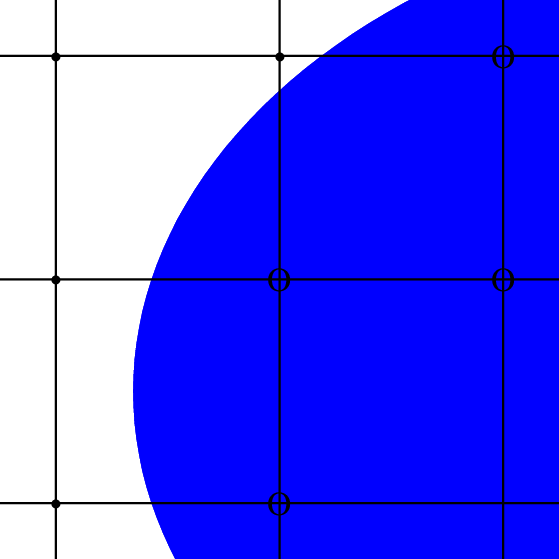
\includegraphics[width=5cm]{../pics/fdo}
}
\centerline{(a) \hspace{7cm}(b)}
\vspace{0.5cm}
\centerline{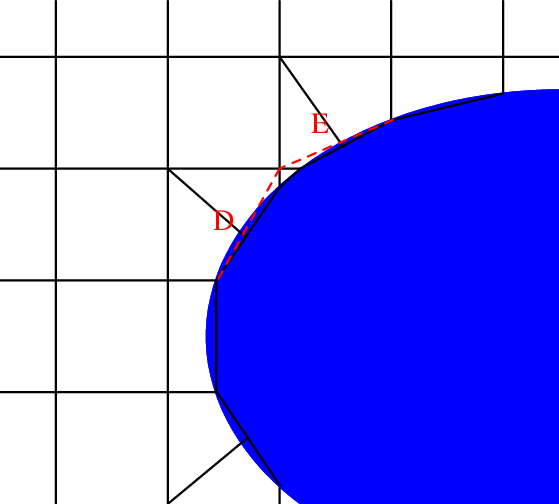
\includegraphics[width=8cm]{../pics/melde} }
\centerline{(c)}
\caption{(a) left top. Cut cell approach to approximating geometry, new edges shown as red dashed lines.
(b) right top.  Immersive approach to boundaries. Cells with open circles at one or more
of their corners have specially modified physics and/or numerics to represent
the fact they intersect the boundary of the body.
(c) bottom. Towards finite elements, all cells are now either $3$-~or~$4$-sided and the mesher
has eliminated a very small cell.
\label{fig:meshd2}}
\end{figure}
\clearpage
\subsection{Cut cells}\label{sec:cutcells}
The idea here is to replace the curved edges of the G1~body with straight lines within
a cell. There is a variant where the straight lines are forced to be parallel to one
or other coordinate, but \Fig{meshd2}(a) shows the situation where this constraint is
not enforced. An immediate issue is that when the body is convex as here, this approach
systematically underestimates its size, which in some situations means the entire
calculation may correspond to different parameters than originally intended.
The bigger problem is that cells cut in this way are not necessarily $4$-sided,
so that again the finite-difference formulae will need modification. Moreover, a 
cell with very short sides has been introduced, which will have serious
implications for the timestep size of an explicit scheme, and the likely
convergence properties of an implicit one. The number of possible cases to treat
is also potentially exponential in the number of corner nodes as discussed in
the next \Sec{immersed}.


%\clearpage
\subsection{Immersed boundaries}\label{sec:immersed}
This approach is illustrated in \Fig{meshd2}(b) for the problem~G1.
Typically a different or modified physical
process is imagined to operate at the nodes just inside the boundary, eg.\ 
in exterior flow problems a large viscous term to damp motion.
One issue that makes these difficult to use in 3-D is that the number
of possible combinations of corner nodes that are separated by the
object boundary is approximately~$2^{N_{cn}}$ where the number of corner
nodes~$N_{cn}=8$ for a cuboid
or other hexahedron. (Obviously the need to treat~$256$ different cases can be reduced
by using rotations to transform to a smaller number of canonical arrangements,
but this coding is relatively tricky.)
Another big issue is the abrupt change in the effective physics which
can make for slow convergence of implicit problems.
%\begin{figure}
%\centerline{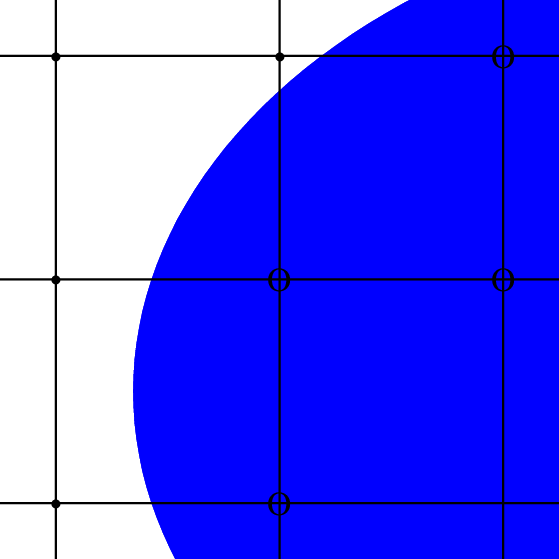
\includegraphics[width=6cm]{../pics/fdo} }
%\caption{Immersive approach to boundaries. Cells with open circles at one or more
%of their corners have specially modified physics and/or numerics to represent
%the fact they intersect the boundary of the body.
%\label{fig:fdo}}
%\end{figure}

%\clearpage
\subsection{Towards Finite Elements}\label{sec:elements}
\Fig{meshd2}(c) shows how the $5$-sided cells can be eliminated by splitting, and in
this case a small cell eliminated, to give a grid composed mostly of quadrilaterals with 
a few triangles.
(In practice, a further demand would be made on the mesher so that the grid-point
shown as just off the body would be moved onto its surface.) Evidently an implicit scheme
should be used because there remain edges which are relatively short. A yet more
sophisticated mesher could be used to give a more uniform distribution of only
quadrilateral cells in the exterior. This would constitute a good finite element mesh\ldots
%\begin{figure}
%\centerline{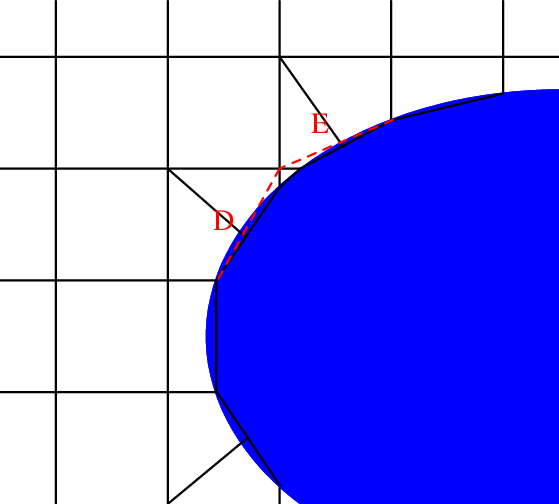
\includegraphics[width=6cm]{../pics/melde} }
%\caption{Towards finite elements, all cells are now $4$-sided and mesher
%has eliminated very small cell.
%\label{fig:melde}}
%\end{figure}
%\begin{equation} \label{eq:EQ}
%{\bf v}^T {\bf b} = {\bf v}^T A {\bf x} = (A^T {\bf v})^T {\bf x} = {\bf g}^T {\bf x}
%\end{equation}

\clearpage
\section{Spectral Elements}\label{sec:sem}
The contrast between finite-difference and finite-element approximation is 
greatest in that finite-difference works in terms of sample points on a regular
grid as indicated in \Sec{geomprob},
whereas finite-element uses an approximation for the solutions interior
to arbitrarily shaped ``elements".
The resulting systems of equations for the discretised fields, eg.\
meaning the finite-difference mesh values
$f_j, j=1,\ldots,N$, also tend to lend themselves to very different methods of
solution. Indeed for simple explicit finite-difference schemes the very concept of 
solving a matrix equation is not required, being replaced by simple
updates in place. This approach tends to be inefficient in finite-elements because
the elements have different sizes, and as remarked in \Sec{geomprob}
the maximum stepsize is restricted by the smallest cells, leading to
implicit schemes that require solution of large systems of linear
equations (sparse matrix equations) for finite element nodal values~$f_j$.

%\clearpage
\subsection{Spectral/hp Elements}\label{sec:semsub}
One justification for use of the term~`spectral' in this context is that early
experiments were made with Fourier series approximations within
the elements. Thus when difficulties were encountered with this
`spectrally accurate' approach and polynomials replaced the trigonometric
functions, the terminology `spectral' was retained to emphasise that high order
polynomials could achieve the same level of theoretical accuracy.

The~$hp$ in the name simply indicates by the~$h$ that finite elements of
very different spatial sizes are allowed and by the~$p$ that arbitrarily
large polynomial orders~$p$ may be exploited. Spectral accuracy may
conceived of as the limiting result $p\rightarrow\infty$, although
in practice the order~$p$ seldom exceeds~$10$.

\begin{figure}[h]
\centerline{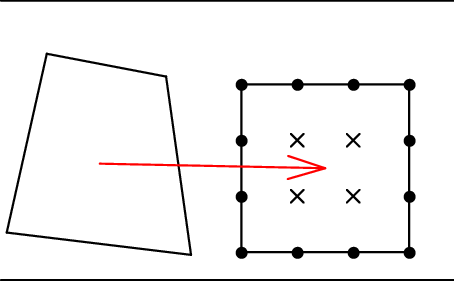
\includegraphics[width=6cm]{../pics/mapquad}
\hspace{1cm}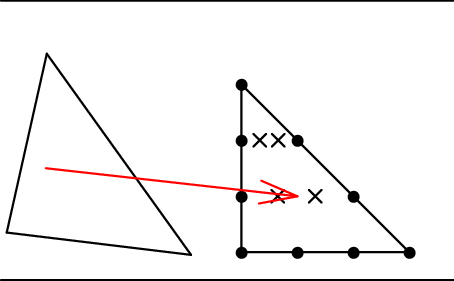
\includegraphics[width=6cm]{../pics/maptri}}
\centerline{(a) \hspace{7cm} (b)}
\caption{An arbitrary planar quadrilateral is mapped to the
unit square (a) and a triangle to a reference triangle (b).
\label{fig:maps}}
\end{figure}

Since the publication of the book by Karniadakis and Sherwin, %\cite{karniadakissherwin}
spectral/hp element has tended to taken on a more specific meaning, namely the use
of Lagrangian interpolation polynomials with nodes at certain specific
`Gauss' points in the elements. Each coordinate direction is treated
separately in this way, and different shaped elements are mapped to
squares or cubes of unit sidelength in order for it to work, see \Fig{maps}.
A key point
is that the mapping between `reference space' and real space can be singular
without disaster for the overall algorithm, thus elements
which are triangles and prisms in real space may be accommodated,
see \Fig{maps}(b).

\begin{figure}[h]
\centerline{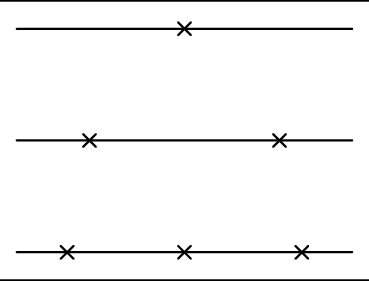
\includegraphics[width=6cm]{../pics/gauxpts}
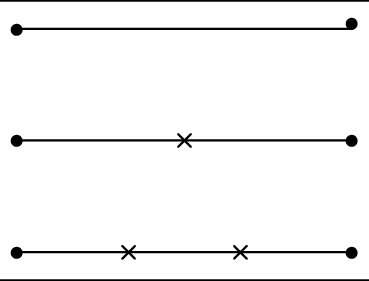
\includegraphics[width=6cm]{../pics/gaulob} }
\centerline{(a) \hspace{7cm} (b)}
\caption{(a) left, intervals marked with Gauss points~$x_{Gj}$
for integrations using respectively from top to bottom, totals of $1$, $2$ and~$3$ samples.
(b) right, are indicated the Gauss-Lobatto points 
for integrations using respectively from top to bottom, totals of $2$, $3$ and~$4$ samples.
\label{fig:gausspts}}
\end{figure}

Gauss points answer the question about the least number of samples
needed to integrate a polynomial of given order over an interval, by giving the
locations of the sample points, and corresponding weights. If only 
one sample point is used, then this should obviously be at the centre
of the interval, but if two are used, it turns out they should be
located at $x=\pm G_1 = \pm 0.577\,350$ when the interval is $-1 \leq x \leq 1$,
and similarly for three points $x=0$, $x=\pm G_2 = \pm 0.774\,597$,
see \Fig{gausspts}(a).
As an aside, this last example implies for the mapped spectral/hp element, three basis functions
which as Lagrangian interpolants are respectively proportional to
\begin{equation} \label{eq:lagpoly}
(x+G_2)x,\;\; x(x-G_2),\;\mbox{and}\; (x+G_2)(x-G_2)
\end{equation}
The general Gauss quadrature formula for integrating a polynomial is
\begin{equation} \label{eq:gaussint}
\int_{-1}^{+1} p(x) dx = \sum_{j=1}^{n} w_{Gj} p(x_{Gj}) 
\end{equation}
where $p(x)$ is the polynomial, $x_{Gj},j=1,\ldots n$ are Gauss points and
$w_{Gj}$ are the corresponding weights, which are tabulated in
numerical analysis texts such as Stoer and Bulirsch. %\cite[\S\,3.6]{stoerbulirsch}
Since the latter points and weights
represent $2n$~degrees of freedom, it turns out that polynomials of order
up to~$2n-1$ can always be integrated exactly in this manner.

However, the better finite element approximations seemingly always
involve placing nodes at element edges, so it becomes necessary to work
with the so-called Gauss-Lobatto points that give maximum accuracy when two of
the $x_{Gj}$ are forced to lie at the interval ends~$x=\pm 1$,
see \Fig{gausspts}(b).  These points
are tabulated by Boyd. %\cite[Appendix F10]{boyd}

\clearpage
\subsection{Working with Spectral/hp Elements}\label{sec:semwork}
Establishing the convergence properties of finite element methods generally requires use of
much heavier mathematics than finite-difference, so this section only touches on key
issues. The most basic operation for discretising partial differential equations
is forming the partial derivative~$\partial f/\partial x$.

Suppose that spectral/hp
elements provide a basis~$\chi_j$, so that a field~$f(x)$ may be represented
\begin{equation}
f(x) = \sum_j f_j \chi_j(x)
\end{equation}
and its derivative has coefficients $f'_j$, then 
\begin{equation}
 \frac{\partial f}{\partial x}= \sum_j f'_j \chi_j(x) \approx \sum_j f_j \frac{\partial \chi_j}{\partial x}
\end{equation}
If $\chi_j(x)$ is a polynomial, then clearly the two discrete expressions
cannot be equal pointwise, but they can be equated in the weak sense.
This is to be interpreted as meaning that the two must have the same
inner product with every member of the basis~$\chi_i, i=1,\ldots N$
\begin{eqnarray}\label{eq:weakdx}
\sum_j f'_j \langle \chi_j, \chi_i \rangle & = & \sum_j f_j \langle \frac{\partial \chi_j}{\partial x}, \chi_i \rangle, \;\; \mbox{ each } i\\
\mbox{where the mass matrix } M_{ij}=\langle \chi_j, \chi_i \rangle & = &  \int_{a}^{b} \chi_j(x) \chi_i(x) dx
\label{eq:inprod}
\end{eqnarray}
Now the significance of interpolation at the Gauss points becomes apparent
since by construction each Lagrange interpolant~$\chi_j$  vanishes at all but one
of these points, which not only reduces
the number of arithmetic operations required to evaluate the mass matrix,
but means that Gauss point interpolation also \emph{diagonalises} the matrix.
%is diagonal, requiring no special inversion techniques.

\clearpage
\subsection{Galerkin versus Discontinuous Galerkin with Spectral/hp Elements}\label{sec:gvsdg}

\begin{figure}
\centerline{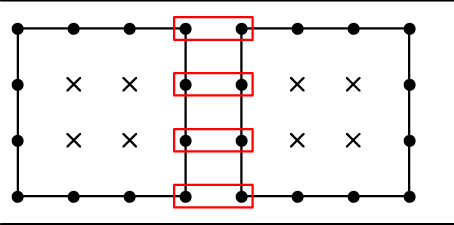
\includegraphics[width=12cm]{../pics/gaulob2d}}
\caption{This shows the locations of Gauss-Lobatto points
on two adjacent reference squares, with the positions of edge nodes
marked using circles, and interior nodes as crosses. In the
usual Galerkin formulation the edge nodes within each red box
have a shared value, whereas in Discontinuous Galerkin these values
are allowed to differ, even though they represent the same point.
\label{fig:gaulob2d}}
\end{figure}
The description of the preceding \Sec{semwork} regarding the
mass matrix has been a little misleading, since
with regular Gauss points, the nodes within each element are effectively decoupled
from those in all other elements, so a practical calculation of $f'_j$
accounting for boundary conditions would not be possible.
%so a realistic calculation would  soon take values
%that almost certainly diverged from one element to another.
Within the standard spectral/hp element
usage of Gauss-Lobatto points, the edge nodes have a special status. The classical
Galerkin formulation implies that the edge nodal value is shared between
at least two elements (more at corners of 2-D elements etc.), see \Fig{gaulob2d},
which has the
effect of coupling this pair of elements together and hence ultimately every node of
every element. (In practice to save storage, the shared nodal value
is saved only once.) However, there is another
option for a surprisingly wide class of problems, which is to allow different
values at these edge nodes in the different elements, even though they correspond
to the same point in space. Typically the (nodal values on different) elements 
are then linked only by means of a flux
condition, giving the Discontinuous Galerkin~(DG) method, so-called for
the obvious reason. 

It is worth commenting on the complementarity of  the finite-element approach relative to finite-difference,
for even though spectral/hp element gives at best  a continuous approximation
to~$f(x)$ at inter-element boundaries, the order of convergence measured in the
energy norm will be of high polynomial order~$p$ in the space variable. 
Crudely speaking, for finite-element, large errors at isolated points are swamped by the accurate integrals
taken over the rest of the interval (and analogously in higher dimensions). Compare
finite-differences, where high order is only enforced at isolated grid-points.

In contrast to other finite-element polynomial bases, transient calculations
with spectral elements do not necessarily require a matrix inversion. However,
integrals such as the right-hand-side of \Eq{weakdx} do couple different elements and thus to
avoid timestep restrictions on a mesh with a wide range of sizes,
will have to be treated at least partly implicitly.
However, the spectral element formulation is here such that if the edge nodal values are known
then the values at the internal modes may be constructed from them. Thus the matrix
equation for implicit time advance that includes the discrete~$\partial /\partial x$ operator,
need only be solved for the edge nodes, at a massive reduction in cost for
high order elements, as highlighted by
Karniadakis and Sherwin.  %\cite[\S\,4.2.3]{karniadakissherwin}
It was not initially realised that the just-described `static condensation' approach to
inverting spectral element matrices could also be extended to Discontinuous
Galerkin, and the ultimate realisation led to the Hybridisable Discontinuous
Galerkin or HDG~algorithm. 

It emerges that HDG and Galerkin methods may be competitive in many problems
involving fluxes. The discontinuity in HDG makes for robustness in 
situations where the physics may support discontinuous solutions,
eg.\ when solving transport equations with practically no dissipation.
On the other hand the discontinuity comes at considerable cost in storage
for there is not just duplication at edge nodes, but the replacement of
one value needed in the Galerkin formulation
by $8$~field values at say, the corners of hexahedral elements.
For practical values of~$p$, the storage overhead of HDG is at least~$50$\,\%,
although this can often be offset by exceptionally large rates of
convergence (`superconvergence') at special nodes.

%Studies indicate that the balance between HDG and Galerkin
%is so fine in classical hydrodynamics
%that it is down to how the (reduced size) matrix problem is solved,
%specifically the selection of preconditioner. %\cite{Ya16ToCG}.







\clearpage
\section{Sparse Matrices}\label{sec:sparse}
For explicit schemes, there is a simple physical argument that, in the case
of advection with speed~$u$, the timestep is restricted by the size of the mesh.
Clearly, information about the presence of a disturbance should travel a distance
$u t$ in a time~$t$. However for an explicit scheme, in one timestep~$\Delta t$,
information will propagate a distance equal to
the mesh-spacing of size~$h$. If $u \Delta t=h$, this is perfect,
and if $u \Delta t<h$, more timesteps may simply be taken so that the value
at the neighbouring point is correctly updated at time $t=h/u$.
However if $u \Delta t>h$, then information is propagating too fast from one
timestep to another, hence disturbances from increasingly unphysically large
distances upstream pile up to produce numerical instability.
Indeed it is found in practice that instability may be expected
wherever $\Delta t>h/u$ on a non-uniform mesh. For a finite element mesh which has been
locally refined say by a factor of~$10$ to account for a boundary layer
or similar feature, this implies great inefficiency when most of the other elements
could otherwise have been advanced at a much faster rate.

The most popular way around the difficulty is to
allow information to flow a distance of many mesh-spacings at each timestep, implying that 
all the nodes need to be connected. This leads to the need to
solve large linear systems of equations 
\begin{equation} \label{eq:mat}
A{\bf x} = {\bf b}
\end{equation}
for the new nodal values~$f_j$ formed into a vector~${\bf x}$,
representing the implicit approach to time-stepping. $A$ is the
matrix that does not the connecting/coupling and the right-hand-side~${\bf b}$
will include information about the present values of~$f_j$.

Now suppose that information~$f_j$, $g_j$, $h_j \ldots$ about several different
species is to be advanced at the same time. At this point the idea of information
propagation is strongly suggestive that all the fields should be formed into~${\bf x}$,
with the ordering
\begin{equation} \label{eq:close}
f_1,g_1,h_1,\ldots, f_2,g_2,h_2,\ldots,f_3,g_3,h_3,\ldots\ldots
\end{equation}
leading to the so-called tight-coupled update, see \Fig{tight}.
\begin{figure}
\centerline{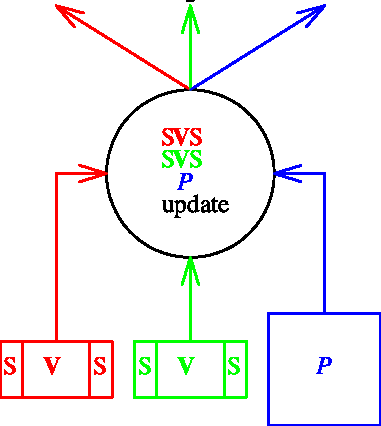
\includegraphics[width=10cm]{../pics/fvpups}}
\caption{Tight-coupled update of $3$~different species indicated by the different colours.
The first two species have a fluid representation consisting of two scalar fields
of density and temperature, and a velocity vector field. The third species~$P$
consists of particles. 
\label{fig:tight}}
\end{figure}

The natural alternative is loose-coupling, where not only is the ordering
\begin{equation} \label{eq:loose}
f_1,f_2,f_3,\ldots, g_1,g_2,g_3,\ldots,h_1,h_2,h_3,\ldots\ldots
\end{equation}
but separate smaller linear systems $A_f {\bf f}= {\bf b}_f$, 
$A_g {\bf g}= {\bf b}_g$, $A_h {\bf h}= {\bf b}_h$, \ldots, are solved in turn,
see \Fig{loose}. It should be evident that the information about updated values
of $h_j$ does not feed into the  new~$f_j$ until there is another cycle 
of updates $A_f {\bf f}= {\bf b}_f$, and then only imperfectly
compared to the tight-coupled approached.


\begin{figure}
\centerline{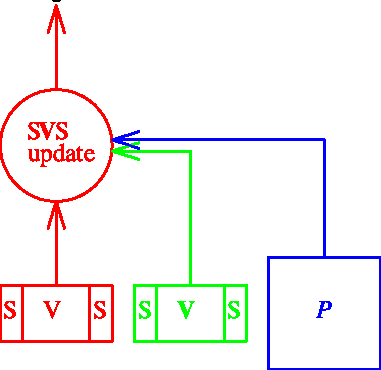
\includegraphics[width=6cm]{../pics/fvms}}
\centerline{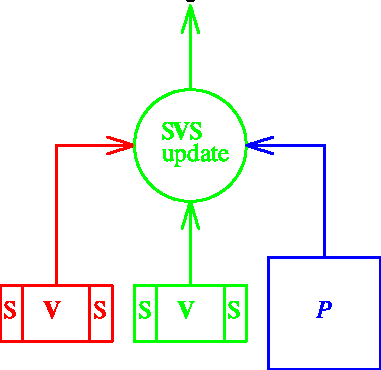
\includegraphics[width=6cm]{../pics/fvps}}
\centerline{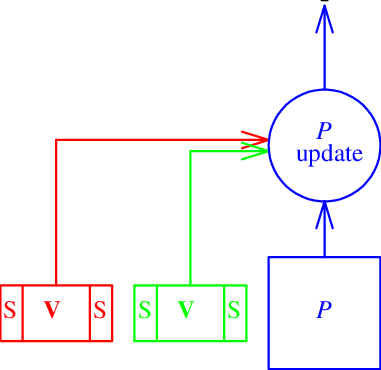
\includegraphics[width=6cm]{../pics/pups}}
\caption{Loose-coupled update of $3$~different species indicated by the different colours.
The first two species have a fluid representation consisting of two scalar fields
of density and temperature, and a velocity vector field. The third species~$P$
consists of particles.  As time increases down the page, first one fluid species
is updated, then the other, finally the particles are updated and the cycle repeats.
\label{fig:loose}}
\end{figure}

The matrix~$A$ will generally
be sparse, with most entries equal to zero, even when `static condensation'
as described in \Sec{sem} has been used to reduce the number of entries in~${\bf x}$
for Galerkin and to give HDG schemes. Since the finite elements will \emph{not} normally
be arranged in a regular pattern, the solution of the linear algebra
problem will have to be obtained by iteration.
These iterations are expected to benefit from appropriate matrix preconditioning, ie.\
algorithms which are mathematically equivalent to forming the 
matrix product $M=C^{-1}A$ so that $M{\bf x}=C^{-1}{\bf b}$ is easier to solve,
typically because iteration proceeds faster as $M$ is closer to a diagonal matrix.
Studies indicate that the balance between HDG and Galerkin
in terms of cost is so fine in classical hydrodynamics
that it is down to how the (reduced size) matrix problem is solved,
specifically the selection of preconditioner~$C$. %\cite{Ya16ToCG}.
Selection of preconditioners is generally regarded as an art.

Since finite elements are widely used in practical applications, much
research has been developed for the solution of the large, sparse
matrix problems which result. Local iterations, such as the Jacobi or Gauss-Seidel
typically taught in introductory courses, have rates of convergence limited
by the rate of information propagation just like the explicit schemes discussed above.
More efficient techniques are available such as (preconditioned) Conjugate Gradients,
which is `unreasonably effective' especially for the Poisson and similar
elliptic problems, and (preconditioned) Krylov methods of which GMRES is the
most popular for other types of physical model, see for example
van der Vorst's book. %~\cite{vandervorst}.
There are a number of practical considerations when it comes to implementing
these algorithms on computing hardware, particularly in relation to 
storage. Generally, forming the complete matrices such as~$A$ and $C^{-1}A$
is avoided as far possible, their entries may be only generated as required
and ideally only an algorithm specified for the action of the preconditioner.

Most attention has so far been paid to the solving the smaller subsystems
eg.\ $A_f {\bf f}= {\bf b}_f$ of the loose-coupling problem. Each can be
treated separately and the basic structures, vectors and sparse matrices of fixed size,
are features of most scientific packages and correspondingly often identified
by vendors for optimised implementation. In contrast,
solving the tight-coupled problem, especially where particle information is
involved, would benefit from further investigation.








\clearpage
%\section{Summary}\label{sec:summ}
%The requirements capture exercise did not raise any significant issues that
had not been anticipated in the Science Plan~\cite{sciplan}.
Concerning modelling and software, there was remarkably little dissension.
The question of the physics to be included has been settled in the
short term  by the need to align with the E-TASC projects on edge modelling.
Longer term there are questions still to be resolved concerning the
details of the gyroaveraged kinetic (or other kinetic) model to be employed,
the inclusion of special relativistic effects, plasma chemistry, 
and for example whether the PFC boundaries should be allowed to `melt',
and whether particle dynamics within the top layers of PFCs should be included.

There is still a debate about how best to deal with situations when the software
even at the Exascale is incapable of resolving boundary or internal layers.
A feature of the lower order (Patankar) fd scheme is that it can be
formulated so that in an implicit time advance of a field advection-diffusion equation,
it acts a contraction mapping on the field, ie.\ it converges to a single, finite solution,
regardless of lack of layer resolution or of size of timestep. Under such circumstances, a spectral
scheme may fail completely cf.\ the dispersion analyses of say Ainsworth et al~\cite{Ai09Disp}
and more recently for spectral/hp element schemes in the Galerkin~\cite{Mo16Eige} and 
discontinuous Galerkin~\cite{Mo15line} contexts,
and users generally prefer an answer to none at all.
Of course, it may be argued that a manifestly erroneous result without an accuracy estimate
will not be used to action large procurements, but in any event it would be better
for the spectral scheme to produce a result at increasingly extreme parameters.

There are a number of ways to achieve this, the most obvious' being the use of
explicit artifical viscosity,
to broaden thinner layers or small features to the
point where full spectral accuracy is achievable.
Different options have been explored, of
which the most robust appears to be `DG-mimicking spectral vanishing viscosity'~ (SVV), see ref~\cite{Mo19Spat}.
Fernandez et al~\cite{Fe19Nonm} specifically addresses robustness when mesh resolution becomes poor..

A better approach from the point-of-view
of accuracy is to insert more resolution (more elements or increased order polynomials)
where aliasing error has been detected. This has its limitations in terms of cost,
but there are also practical issues concerning refinement that still need investigation.
Some of these latter points might be more easily addressed by reformulating the problem 
in terms of a variational approach and/or using the Lie derivative formulation~\cite{La03prac}.
It was anticipated that these could be addressed in the cross-cutting programme.

Interaction with a reactor design framework awaits better definition of data structures
for such tools. There seems no reason however why this should not be addressed inside-out,
as regardless, techniques have to be produced for moving data at the Exascale.

Subject to the above qualifications, the production of proxyapps should proceed in Y2 as indicated
in the Activities Plan~\cite{y12acts}, viz.\ a larger task :
\begin{itemize}
\item to define a referent physics model for the tokamak edge region, accounting
for magnetised plasma behaviour in the presence of significant numbers of neutral atoms and molecules, allowing for
radiation and chemical reactions, and identifying important wall interactions such as sheath formation.
\end{itemize}
This task will be expected to interact with other tasks to ensure feasible implementation.
It is desirable that theroretical support be provided for the EBC pilot code development,
which is a 2-D fluid model, as well as for the 1-D fluid cases with kinetic effects explicitly
listed below.

The candidate algorithms are expected to employ spectral finite element and particle representations.
There are 5 tasks for which advanced mathematical skills will be important:
\begin{enumerate}
\item  to assess performance of spectral elements for \nep \ 
\item  to examine the optimal replacement of plasma species properties
represented on high-order spatially accurate meshes by a particle representation and vice versa.
\item  to study uncertainty quantification (UQ) techniques for \nep \ .
\item  to study model order reduction techniques for \nep \ .
\item  to investigate matrix-preconditioning techniques for \nep \ .
\end{enumerate}
There are 4 tasks to develop proxy-apps for \nep \  of demonstrable, high accuracy
in challenging test-cases, namely :
\begin{enumerate}
\item  2-D model of anisotropic heat transport.
\item  2-D elliptic solver in complex geometry.
\item  1-D fluid solver with simplified physics but with UQ and realistic boundary conditions.
\item  1-D plasma model incorporating velocity space effects.
\end{enumerate}
There are 2  tasks concerning software engineering for \nep \ 
\begin{enumerate}
\item  to investigate DSL and code generation techniques for \nep \ .
\item  to investigate, in collaboration with UKAEA staff, data structures and design patterns for \nep \ .
\end{enumerate}

The Science Plan~\cite{sciplan} shows how the proxyapps should feed into the $5$-year development.
All the tasks may use any identified software packages including
commercial software as part of the demonstration process, provided a feasible route to producing code
freely usable by \nep \  is clearly indicated. It will obviously be better if a task
is linked to the delivery of a proxy-app.




%\section*{Acknowledgement}\label{sec:ackn}
%This work is a version, with citations removed, of notes
intended for publication by the author as part of an advanced
textbook on computational physics.


%\section*{References}
%\bibliographystyle{unsrt}
%\bibliography{../bib/new,../bib/waynes,../bib/misc,../bib/warv,../bib/neuts,../bib/reac,../bib/exc,../bib/active,../bib/dg1srt}

\end{document}
